% Created by tikzDevice version 0.10.1 on 2017-09-05 18:24:29
% !TEX encoding = UTF-8 Unicode
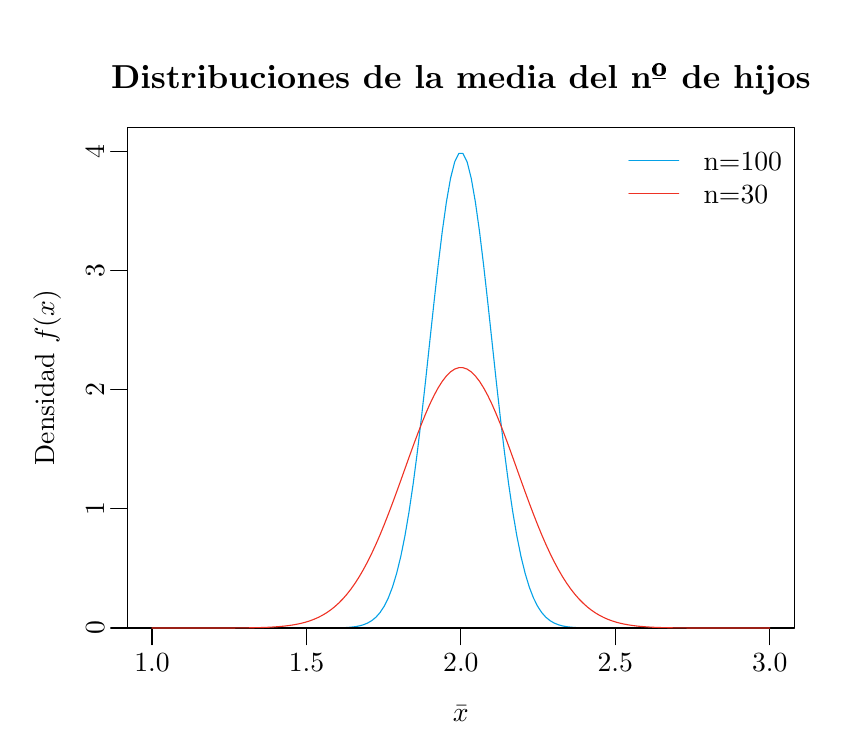
\begin{tikzpicture}[x=1pt,y=1pt]
\definecolor{fillColor}{RGB}{255,255,255}
\path[use as bounding box,fill=fillColor,fill opacity=0.00] (0,0) rectangle (289.08,252.94);
\begin{scope}
\path[clip] ( 36.00, 36.00) rectangle (277.08,216.94);
\definecolor{drawColor}{RGB}{5,161,230}

\path[draw=drawColor,line width= 0.4pt,line join=round,line cap=round] ( 44.93, 36.00) --
	( 46.43, 36.00) --
	( 47.93, 36.00) --
	( 49.42, 36.00) --
	( 50.92, 36.00) --
	( 52.42, 36.00) --
	( 53.92, 36.00) --
	( 55.42, 36.00) --
	( 56.91, 36.00) --
	( 58.41, 36.00) --
	( 59.91, 36.00) --
	( 61.41, 36.00) --
	( 62.91, 36.00) --
	( 64.40, 36.00) --
	( 65.90, 36.00) --
	( 67.40, 36.00) --
	( 68.90, 36.00) --
	( 70.40, 36.00) --
	( 71.90, 36.00) --
	( 73.39, 36.00) --
	( 74.89, 36.00) --
	( 76.39, 36.00) --
	( 77.89, 36.00) --
	( 79.39, 36.00) --
	( 80.88, 36.00) --
	( 82.38, 36.00) --
	( 83.88, 36.00) --
	( 85.38, 36.00) --
	( 86.88, 36.00) --
	( 88.37, 36.00) --
	( 89.87, 36.00) --
	( 91.37, 36.00) --
	( 92.87, 36.00) --
	( 94.37, 36.00) --
	( 95.87, 36.00) --
	( 97.36, 36.00) --
	( 98.86, 36.00) --
	(100.36, 36.00) --
	(101.86, 36.00) --
	(103.36, 36.00) --
	(104.85, 36.00) --
	(106.35, 36.01) --
	(107.85, 36.01) --
	(109.35, 36.02) --
	(110.85, 36.04) --
	(112.34, 36.07) --
	(113.84, 36.11) --
	(115.34, 36.19) --
	(116.84, 36.31) --
	(118.34, 36.49) --
	(119.84, 36.77) --
	(121.33, 37.19) --
	(122.83, 37.80) --
	(124.33, 38.67) --
	(125.83, 39.90) --
	(127.33, 41.59) --
	(128.82, 43.87) --
	(130.32, 46.89) --
	(131.82, 50.79) --
	(133.32, 55.74) --
	(134.82, 61.86) --
	(136.32, 69.28) --
	(137.81, 78.06) --
	(139.31, 88.21) --
	(140.81, 99.66) --
	(142.31,112.23) --
	(143.81,125.65) --
	(145.30,139.55) --
	(146.80,153.47) --
	(148.30,166.88) --
	(149.80,179.21) --
	(151.30,189.91) --
	(152.79,198.46) --
	(154.29,204.42) --
	(155.79,207.49) --
	(157.29,207.49) --
	(158.79,204.42) --
	(160.29,198.46) --
	(161.78,189.91) --
	(163.28,179.21) --
	(164.78,166.88) --
	(166.28,153.47) --
	(167.78,139.55) --
	(169.27,125.65) --
	(170.77,112.23) --
	(172.27, 99.66) --
	(173.77, 88.21) --
	(175.27, 78.06) --
	(176.76, 69.28) --
	(178.26, 61.86) --
	(179.76, 55.74) --
	(181.26, 50.79) --
	(182.76, 46.89) --
	(184.26, 43.87) --
	(185.75, 41.59) --
	(187.25, 39.90) --
	(188.75, 38.67) --
	(190.25, 37.80) --
	(191.75, 37.19) --
	(193.24, 36.77) --
	(194.74, 36.49) --
	(196.24, 36.31) --
	(197.74, 36.19) --
	(199.24, 36.11) --
	(200.74, 36.07) --
	(202.23, 36.04) --
	(203.73, 36.02) --
	(205.23, 36.01) --
	(206.73, 36.01) --
	(208.23, 36.00) --
	(209.72, 36.00) --
	(211.22, 36.00) --
	(212.72, 36.00) --
	(214.22, 36.00) --
	(215.72, 36.00) --
	(217.21, 36.00) --
	(218.71, 36.00) --
	(220.21, 36.00) --
	(221.71, 36.00) --
	(223.21, 36.00) --
	(224.71, 36.00) --
	(226.20, 36.00) --
	(227.70, 36.00) --
	(229.20, 36.00) --
	(230.70, 36.00) --
	(232.20, 36.00) --
	(233.69, 36.00) --
	(235.19, 36.00) --
	(236.69, 36.00) --
	(238.19, 36.00) --
	(239.69, 36.00) --
	(241.18, 36.00) --
	(242.68, 36.00) --
	(244.18, 36.00) --
	(245.68, 36.00) --
	(247.18, 36.00) --
	(248.68, 36.00) --
	(250.17, 36.00) --
	(251.67, 36.00) --
	(253.17, 36.00) --
	(254.67, 36.00) --
	(256.17, 36.00) --
	(257.66, 36.00) --
	(259.16, 36.00) --
	(260.66, 36.00) --
	(262.16, 36.00) --
	(263.66, 36.00) --
	(265.15, 36.00) --
	(266.65, 36.00) --
	(268.15, 36.00);
\end{scope}
\begin{scope}
\path[clip] (  0.00,  0.00) rectangle (289.08,252.94);
\definecolor{drawColor}{RGB}{0,0,0}

\path[draw=drawColor,line width= 0.4pt,line join=round,line cap=round] ( 44.93, 36.00) -- (268.15, 36.00);

\path[draw=drawColor,line width= 0.4pt,line join=round,line cap=round] ( 44.93, 36.00) -- ( 44.93, 30.00);

\path[draw=drawColor,line width= 0.4pt,line join=round,line cap=round] (100.73, 36.00) -- (100.73, 30.00);

\path[draw=drawColor,line width= 0.4pt,line join=round,line cap=round] (156.54, 36.00) -- (156.54, 30.00);

\path[draw=drawColor,line width= 0.4pt,line join=round,line cap=round] (212.35, 36.00) -- (212.35, 30.00);

\path[draw=drawColor,line width= 0.4pt,line join=round,line cap=round] (268.15, 36.00) -- (268.15, 30.00);

\node[text=drawColor,anchor=base,inner sep=0pt, outer sep=0pt, scale=  1.00] at ( 44.93, 20.40) {1.0};

\node[text=drawColor,anchor=base,inner sep=0pt, outer sep=0pt, scale=  1.00] at (100.73, 20.40) {1.5};

\node[text=drawColor,anchor=base,inner sep=0pt, outer sep=0pt, scale=  1.00] at (156.54, 20.40) {2.0};

\node[text=drawColor,anchor=base,inner sep=0pt, outer sep=0pt, scale=  1.00] at (212.35, 20.40) {2.5};

\node[text=drawColor,anchor=base,inner sep=0pt, outer sep=0pt, scale=  1.00] at (268.15, 20.40) {3.0};

\path[draw=drawColor,line width= 0.4pt,line join=round,line cap=round] ( 36.00, 36.00) -- ( 36.00,208.33);

\path[draw=drawColor,line width= 0.4pt,line join=round,line cap=round] ( 36.00, 36.00) -- ( 30.00, 36.00);

\path[draw=drawColor,line width= 0.4pt,line join=round,line cap=round] ( 36.00, 79.08) -- ( 30.00, 79.08);

\path[draw=drawColor,line width= 0.4pt,line join=round,line cap=round] ( 36.00,122.16) -- ( 30.00,122.16);

\path[draw=drawColor,line width= 0.4pt,line join=round,line cap=round] ( 36.00,165.25) -- ( 30.00,165.25);

\path[draw=drawColor,line width= 0.4pt,line join=round,line cap=round] ( 36.00,208.33) -- ( 30.00,208.33);

\node[text=drawColor,rotate= 90.00,anchor=base,inner sep=0pt, outer sep=0pt, scale=  1.00] at ( 27.60, 36.00) {0};

\node[text=drawColor,rotate= 90.00,anchor=base,inner sep=0pt, outer sep=0pt, scale=  1.00] at ( 27.60, 79.08) {1};

\node[text=drawColor,rotate= 90.00,anchor=base,inner sep=0pt, outer sep=0pt, scale=  1.00] at ( 27.60,122.16) {2};

\node[text=drawColor,rotate= 90.00,anchor=base,inner sep=0pt, outer sep=0pt, scale=  1.00] at ( 27.60,165.25) {3};

\node[text=drawColor,rotate= 90.00,anchor=base,inner sep=0pt, outer sep=0pt, scale=  1.00] at ( 27.60,208.33) {4};

\path[draw=drawColor,line width= 0.4pt,line join=round,line cap=round] ( 36.00, 36.00) --
	(277.08, 36.00) --
	(277.08,216.94) --
	( 36.00,216.94) --
	( 36.00, 36.00);
\end{scope}
\begin{scope}
\path[clip] (  0.00,  0.00) rectangle (289.08,252.94);
\definecolor{drawColor}{RGB}{0,0,0}

\node[text=drawColor,anchor=base,inner sep=0pt, outer sep=0pt, scale=  1.20] at (156.54,230.80) {\bfseries Distribuciones de la media del nº de hijos};

\node[text=drawColor,anchor=base,inner sep=0pt, outer sep=0pt, scale=  1.00] at (156.54,  2.40) {$\bar x$};

\node[text=drawColor,rotate= 90.00,anchor=base,inner sep=0pt, outer sep=0pt, scale=  1.00] at (  9.60,126.47) {Densidad $f(x)$};
\end{scope}
\begin{scope}
\path[clip] ( 36.00, 36.00) rectangle (277.08,216.94);
\definecolor{drawColor}{RGB}{238,50,36}

\path[draw=drawColor,line width= 0.4pt,line join=round,line cap=round] ( 44.93, 36.00) --
	( 46.43, 36.00) --
	( 47.93, 36.00) --
	( 49.42, 36.00) --
	( 50.92, 36.00) --
	( 52.42, 36.00) --
	( 53.92, 36.00) --
	( 55.42, 36.00) --
	( 56.91, 36.00) --
	( 58.41, 36.00) --
	( 59.91, 36.00) --
	( 61.41, 36.00) --
	( 62.91, 36.00) --
	( 64.40, 36.00) --
	( 65.90, 36.00) --
	( 67.40, 36.01) --
	( 68.90, 36.01) --
	( 70.40, 36.01) --
	( 71.90, 36.02) --
	( 73.39, 36.02) --
	( 74.89, 36.03) --
	( 76.39, 36.04) --
	( 77.89, 36.05) --
	( 79.39, 36.07) --
	( 80.88, 36.10) --
	( 82.38, 36.13) --
	( 83.88, 36.16) --
	( 85.38, 36.21) --
	( 86.88, 36.27) --
	( 88.37, 36.35) --
	( 89.87, 36.45) --
	( 91.37, 36.57) --
	( 92.87, 36.71) --
	( 94.37, 36.90) --
	( 95.87, 37.12) --
	( 97.36, 37.39) --
	( 98.86, 37.71) --
	(100.36, 38.10) --
	(101.86, 38.57) --
	(103.36, 39.12) --
	(104.85, 39.77) --
	(106.35, 40.53) --
	(107.85, 41.42) --
	(109.35, 42.44) --
	(110.85, 43.62) --
	(112.34, 44.96) --
	(113.84, 46.48) --
	(115.34, 48.19) --
	(116.84, 50.11) --
	(118.34, 52.24) --
	(119.84, 54.59) --
	(121.33, 57.16) --
	(122.83, 59.96) --
	(124.33, 62.99) --
	(125.83, 66.24) --
	(127.33, 69.69) --
	(128.82, 73.33) --
	(130.32, 77.15) --
	(131.82, 81.10) --
	(133.32, 85.18) --
	(134.82, 89.33) --
	(136.32, 93.53) --
	(137.81, 97.71) --
	(139.31,101.85) --
	(140.81,105.88) --
	(142.31,109.76) --
	(143.81,113.44) --
	(145.30,116.86) --
	(146.80,119.98) --
	(148.30,122.75) --
	(149.80,125.13) --
	(151.30,127.07) --
	(152.79,128.56) --
	(154.29,129.57) --
	(155.79,130.08) --
	(157.29,130.08) --
	(158.79,129.57) --
	(160.29,128.56) --
	(161.78,127.07) --
	(163.28,125.13) --
	(164.78,122.75) --
	(166.28,119.98) --
	(167.78,116.86) --
	(169.27,113.44) --
	(170.77,109.76) --
	(172.27,105.88) --
	(173.77,101.85) --
	(175.27, 97.71) --
	(176.76, 93.53) --
	(178.26, 89.33) --
	(179.76, 85.18) --
	(181.26, 81.10) --
	(182.76, 77.15) --
	(184.26, 73.33) --
	(185.75, 69.69) --
	(187.25, 66.24) --
	(188.75, 62.99) --
	(190.25, 59.96) --
	(191.75, 57.16) --
	(193.24, 54.59) --
	(194.74, 52.24) --
	(196.24, 50.11) --
	(197.74, 48.19) --
	(199.24, 46.48) --
	(200.74, 44.96) --
	(202.23, 43.62) --
	(203.73, 42.44) --
	(205.23, 41.42) --
	(206.73, 40.53) --
	(208.23, 39.77) --
	(209.72, 39.12) --
	(211.22, 38.57) --
	(212.72, 38.10) --
	(214.22, 37.71) --
	(215.72, 37.39) --
	(217.21, 37.12) --
	(218.71, 36.90) --
	(220.21, 36.71) --
	(221.71, 36.57) --
	(223.21, 36.45) --
	(224.71, 36.35) --
	(226.20, 36.27) --
	(227.70, 36.21) --
	(229.20, 36.16) --
	(230.70, 36.13) --
	(232.20, 36.10) --
	(233.69, 36.07) --
	(235.19, 36.05) --
	(236.69, 36.04) --
	(238.19, 36.03) --
	(239.69, 36.02) --
	(241.18, 36.02) --
	(242.68, 36.01) --
	(244.18, 36.01) --
	(245.68, 36.01) --
	(247.18, 36.00) --
	(248.68, 36.00) --
	(250.17, 36.00) --
	(251.67, 36.00) --
	(253.17, 36.00) --
	(254.67, 36.00) --
	(256.17, 36.00) --
	(257.66, 36.00) --
	(259.16, 36.00) --
	(260.66, 36.00) --
	(262.16, 36.00) --
	(263.66, 36.00) --
	(265.15, 36.00) --
	(266.65, 36.00) --
	(268.15, 36.00);
\definecolor{drawColor}{RGB}{5,161,230}

\path[draw=drawColor,line width= 0.4pt,line join=round,line cap=round] (217.25,204.94) -- (235.25,204.94);
\definecolor{drawColor}{RGB}{238,50,36}

\path[draw=drawColor,line width= 0.4pt,line join=round,line cap=round] (217.25,192.94) -- (235.25,192.94);
\definecolor{drawColor}{RGB}{0,0,0}

\node[text=drawColor,anchor=base west,inner sep=0pt, outer sep=0pt, scale=  1.00] at (244.25,201.50) {n=100};

\node[text=drawColor,anchor=base west,inner sep=0pt, outer sep=0pt, scale=  1.00] at (244.25,189.50) {n=30};
\end{scope}
\end{tikzpicture}
